\documentclass[10pt,ignorenonframetext,,aspectratio=149]{beamer}
\usefonttheme{serif} % use mainfont rather than sansfont for slide text
\setbeamertemplate{caption}[numbered]
\setbeamertemplate{caption label separator}{: }
\setbeamercolor{caption name}{fg=normal text.fg}
\usepackage{lmodern}
\usepackage{amssymb,amsmath}
\usepackage{ifxetex,ifluatex}
\usepackage{fixltx2e} % provides \textsubscript
\ifnum 0\ifxetex 1\fi\ifluatex 1\fi=0 % if pdftex
  \usepackage[T1]{fontenc}
  \usepackage[utf8]{inputenc}
\else % if luatex or xelatex
  \ifxetex
    \usepackage{mathspec}
  \else
    \usepackage{fontspec}
  \fi
  \defaultfontfeatures{Ligatures=TeX,Scale=MatchLowercase}
  \newcommand{\euro}{€}
    \setmainfont[]{Open Sans}
\fi
% use upquote if available, for straight quotes in verbatim environments
\IfFileExists{upquote.sty}{\usepackage{upquote}}{}
% use microtype if available
\IfFileExists{microtype.sty}{%
\usepackage{microtype}
\UseMicrotypeSet[protrusion]{basicmath} % disable protrusion for tt fonts
}{}
\usepackage{graphicx,grffile}
\makeatletter
\def\maxwidth{\ifdim\Gin@nat@width>\linewidth\linewidth\else\Gin@nat@width\fi}
\def\maxheight{\ifdim\Gin@nat@height>\textheight0.8\textheight\else\Gin@nat@height\fi}
\makeatother
% Scale images if necessary, so that they will not overflow the page
% margins by default, and it is still possible to overwrite the defaults
% using explicit options in \includegraphics[width, height, ...]{}
\setkeys{Gin}{width=\maxwidth,height=\maxheight,keepaspectratio}

% Comment these out if you don't want a slide with just the
% part/section/subsection/subsubsection title:
\AtBeginPart{
  \let\insertpartnumber\relax
  \let\partname\relax
  \frame{\partpage}
}
\AtBeginSection{
  \let\insertsectionnumber\relax
  \let\sectionname\relax
  \frame{\sectionpage}
}
\AtBeginSubsection{
  \let\insertsubsectionnumber\relax
  \let\subsectionname\relax
  \frame{\subsectionpage}
}

\setlength{\emergencystretch}{3em}  % prevent overfull lines
\providecommand{\tightlist}{%
  \setlength{\itemsep}{0pt}\setlength{\parskip}{0pt}}
\setcounter{secnumdepth}{0}

\title{Introduction}
\author{Henrique Veras}
\date{}

%% Here's everything I added.
%%--------------------------

\usepackage{graphicx}
\usepackage{rotating}
%\setbeamertemplate{caption}[numbered]
\usepackage{hyperref}
\usepackage{caption}
\usepackage[normalem]{ulem}
%\mode<presentation>
\usepackage{wasysym}
%\usepackage{amsmath}


% Get rid of navigation symbols.
%-------------------------------
\setbeamertemplate{navigation symbols}{}

% Optional institute tags and titlegraphic.
% Do feel free to change the titlegraphic if you don't want it as a Markdown field.
%----------------------------------------------------------------------------------
\institute{PIMES/UFPE}

% \titlegraphic{\includegraphics[width=0.3\paperwidth]{\string~/Dropbox/teaching/clemson-academic.png}} % <-- if you want to know what this looks like without it as a Markdown field. 
% -----------------------------------------------------------------------------------------------------


% Some additional title page adjustments.
%----------------------------------------
\setbeamertemplate{title page}[empty]
%\date{}
\setbeamerfont{subtitle}{size=\small}

\setbeamercovered{transparent}

% Some optional colors. Change or add as you see fit.
%---------------------------------------------------
\definecolor{clemsonpurple}{HTML}{522D80}
 \definecolor{clemsonorange}{HTML}{F66733}
\definecolor{uiucblue}{HTML}{003C7D}
\definecolor{uiucorange}{HTML}{F47F24}


% Some optional color adjustments to Beamer. Change as you see fit.
%------------------------------------------------------------------
\setbeamercolor{frametitle}{fg=clemsonpurple,bg=white}
\setbeamercolor{title}{fg=clemsonpurple,bg=white}
\setbeamercolor{local structure}{fg=clemsonpurple}
\setbeamercolor{section in toc}{fg=clemsonpurple,bg=white}
% \setbeamercolor{subsection in toc}{fg=clemsonorange,bg=white}
\setbeamercolor{footline}{fg=clemsonpurple!50, bg=white}
\setbeamercolor{block title}{fg=clemsonorange,bg=white}


\let\Tiny=\tiny


% Sections and subsections should not get their own damn slide.
%--------------------------------------------------------------
\AtBeginPart{}
\AtBeginSection{}
\AtBeginSubsection{}
\AtBeginSubsubsection{}

% Suppress some of Markdown's weird default vertical spacing.
%------------------------------------------------------------
\setlength{\emergencystretch}{0em}  % prevent overfull lines
\setlength{\parskip}{0pt}


% Allow for those simple two-tone footlines I like. 
% Edit the colors as you see fit.
%--------------------------------------------------
\defbeamertemplate*{footline}{my footline}{%
    \ifnum\insertpagenumber=1
    \hbox{%
        \begin{beamercolorbox}[wd=\paperwidth,ht=.8ex,dp=1ex,center]{}%
      % empty environment to raise height
        \end{beamercolorbox}%
    }%
    \vskip0pt%
    \else%
        \Tiny{%
            \hfill%
		\vspace*{1pt}%
            \insertframenumber/\inserttotalframenumber \hspace*{0.1cm}%
            \newline%
            \color{clemsonpurple}{\rule{\paperwidth}{0.4mm}}\newline%
            \color{clemsonorange}{\rule{\paperwidth}{.4mm}}%
        }%
    \fi%
}

% Various cosmetic things, though I must confess I forget what exactly these do and why I included them.
%-------------------------------------------------------------------------------------------------------
\setbeamercolor{structure}{fg=blue}
\setbeamercolor{local structure}{parent=structure}
\setbeamercolor{item projected}{parent=item,use=item,fg=clemsonpurple,bg=white}
\setbeamercolor{enumerate item}{parent=item}

% Adjust some item elements. More cosmetic things.
%-------------------------------------------------
\setbeamertemplate{itemize item}{\color{clemsonpurple}$\bullet$}
\setbeamertemplate{itemize subitem}{\color{clemsonpurple}\scriptsize{$\bullet$}}
\setbeamertemplate{itemize/enumerate body end}{\vspace{.6\baselineskip}} % So I'm less inclined to use \medskip and \bigskip in Markdown.

% Automatically center images
% ---------------------------
% Note: this is for ![](image.png) images
% Use "fig.align = "center" for R chunks

\usepackage{etoolbox}

\AtBeginDocument{%
  \letcs\oig{@orig\string\includegraphics}%
  \renewcommand<>\includegraphics[2][]{%
    \only#3{%
      {\centering\oig[{#1}]{#2}\par}%
    }%
  }%
}

% I think I've moved to xelatex now. Here's some stuff for that.
% --------------------------------------------------------------
% I could customize/generalize this more but the truth is it works for my circumstances.

\ifxetex
\setbeamerfont{title}{family=\fontspec{Titillium Web}}
\setbeamerfont{frametitle}{family=\fontspec{Titillium Web}}
\usepackage[font=small,skip=0pt]{caption}
 \else
 \fi

% Okay, and begin the actual document...

\begin{document}
\frame{\titlepage}

\hypertarget{econometrics}{%
\section{Econometrics}\label{econometrics}}

\hypertarget{intro}{%
\subsection{Intro}\label{intro}}

\begin{frame}[fragile]{Introduction}
\protect\hypertarget{introduction}{}
What conveys the study of econometrics?

\vfill

The unification of three main areas:

\begin{verbatim}
1.    Statistics
2.    Economic theory
3.    Mathematics
\end{verbatim}

\vfill

``Econometrics conveys application of mathematical statistics and the
tools of statistical inference to the empirical measurement of
relationships postulated by an underlying theory.''
\end{frame}

\hypertarget{the-practice-of-econometrics}{%
\subsection{The practice of
econometrics}\label{the-practice-of-econometrics}}

\begin{frame}{The practice of econometrics}
\protect\hypertarget{the-practice-of-econometrics-1}{}
Theoretical econometrics vs.~applied econometrics

\hspace{3cm}

This course is designed for the applied economist.

\hspace{3cm}

Applied econometric methods will be used for estimation of important
quantities, analysis of economic outcomes such as policy changes,
markets or individual behavior, testing theories, and for forecasting.
\end{frame}

\hypertarget{econometric-modeling}{%
\subsection{Econometric Modeling}\label{econometric-modeling}}

\begin{frame}{Econometric Modeling}
\protect\hypertarget{econometric-modeling-1}{}
Consider the Keynesian consumption function: \(C=f(X)\), where \(X\) is
disposable income.

\vfill

Theoretical postulates: \(dC/dX\) is positive and \(0<dC/dX<1\).

\vfill

Implications:

\begin{enumerate}
\item
  \(MPC>0\)
\item
  \(APC=C/X\) falls with income
\end{enumerate}
\end{frame}

\begin{frame}{Keynes' Consumption Funcion}
\protect\hypertarget{keynes-consumption-funcion}{}
How do we test this theory? \pause

\vfill

Estimate the equation \(C=\alpha + \beta X\) and test whether
\(\alpha>0\) and \(0<\beta<1\).

\vfill

Some points to note:

\begin{enumerate}
\item
  Notice the behavioral aspect of the model.
\item
  The model states an unambiguous and deterministic relationship between
  the dependent and independent variables.
\item
  Models are only simplifications of reality; we need an stochastic
  element.
\item
  A probabilistic model is less precise but more robust!
\end{enumerate}
\end{frame}

\begin{frame}{From the Model to the Real World}
\protect\hypertarget{from-the-model-to-the-real-world}{}
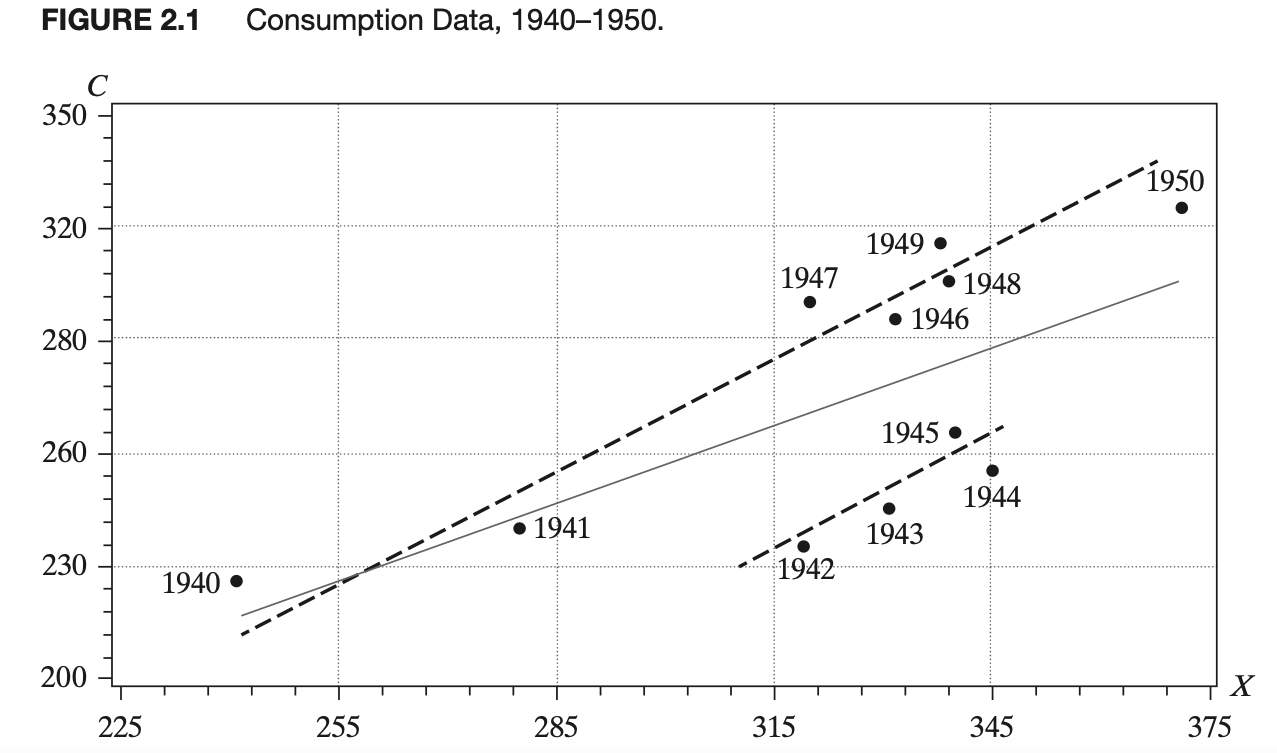
\includegraphics{/Users/henriquefonseca/Desktop/temp/Rmarkdown-practice/henriqueveras.github.io/files/Econometrics/Lecture Notes/1/fig 2.1.PNG}
\end{frame}

\begin{frame}{From the Model to the Real World}
\protect\hypertarget{from-the-model-to-the-real-world-1}{}
The next step is to include a random component: \(C=F(X,\varepsilon)\)

We usually assume an additive relationship.

\vfill

We also need to consider the wartime period into the empirical model.

Here's an empirical model:
\[C=\alpha+\beta X+ d_{waryears}\delta_W+\varepsilon\]
\end{frame}

\begin{frame}{Another Example}
\protect\hypertarget{another-example}{}
How would you model the function \(earnings=f(education)\)?
\end{frame}

\begin{frame}{The Big Data Revolution: Into a new paradigm?}
\protect\hypertarget{the-big-data-revolution-into-a-new-paradigm}{}
Traditional econometrics: Measuring and testing theoretical
relationships

\vspace{1cm}

Can Big Data replace theory?
\end{frame}


\section[]{}
\frame{\small \frametitle{Table of Contents}
\tableofcontents}
\end{document}
